% Section 10: Cosmology
\section{Cosmology}
\label{sec:cosmology}

\subsection{Introduction: The Cosmic Evolution Picture}

UFT cosmology derives cosmic evolution from a single geometric principle:
\begin{itemize}
    \item \textbf{Inflation}: From the transition of spectral dimension from 10D to 4D
    \item \textbf{Dark Energy}: Geometric origin of $\Lambda$
    \item \textbf{Dark Matter}: Primordial black hole remnants
    \item \textbf{Baryogenesis}: Geometric origin of CP violation
\end{itemize}

\subsection{Torsion-Driven Inflation}

\subsubsection{Geometric Mechanism of Inflation}

In UFT, inflation is not driven by a hypothetical inflaton field but by the dimensional transition of spectral dimension.

\begin{insight}[Inflation as Dimensional Transition]
The early universe's high-energy state corresponds to spectral dimension $d_s \approx 10$. As the universe expands and cools, the spectral dimension "freezes" to $d_s = 4$ through torsion field dynamics. This transition manifests as exponential expansion—inflation.
\end{insight}

\subsubsection{Inflaton Field as Spectral Dimension}

The effective inflaton field is the spectral dimension deviation from its low-energy value:
\begin{equation}
    \phi_{\text{inf}}(t) \equiv d_s(t) - 4
\end{equation}

Dynamics driven by torsion field energy density:
\begin{equation}
    \rho_{\text{inf}} = \rho_\tau = \frac{\tau_0^2}{\kappa^2} \cdot f(d_s)
\end{equation}

\subsubsection{Slow-Roll Parameters}

Slow-roll parameters derived from spectral dimension flow:
\begin{equation}
    \epsilon = -\frac{\dot{H}}{H^2} = \frac{3\tau_0^2}{2(d_s - 4)^2}
\end{equation}

As $d_s \to 4$ (approaching dimensional freezing), $\epsilon \to \infty$, slow-roll ends.

\subsection{Spectral Dimension Evolution in the Early Universe}

\subsubsection{Dimensional Transition Dynamics}

The transition of spectral dimension from $d_s = 10$ to $d_s = 4$ follows:
\begin{equation}
    d_s(T) = 4 + \frac{6}{1 + (T/T_c)^2}
\end{equation}

where $T_c \sim 10^{16}$ GeV is the GUT scale.

\begin{figure}[htbp]
\centering
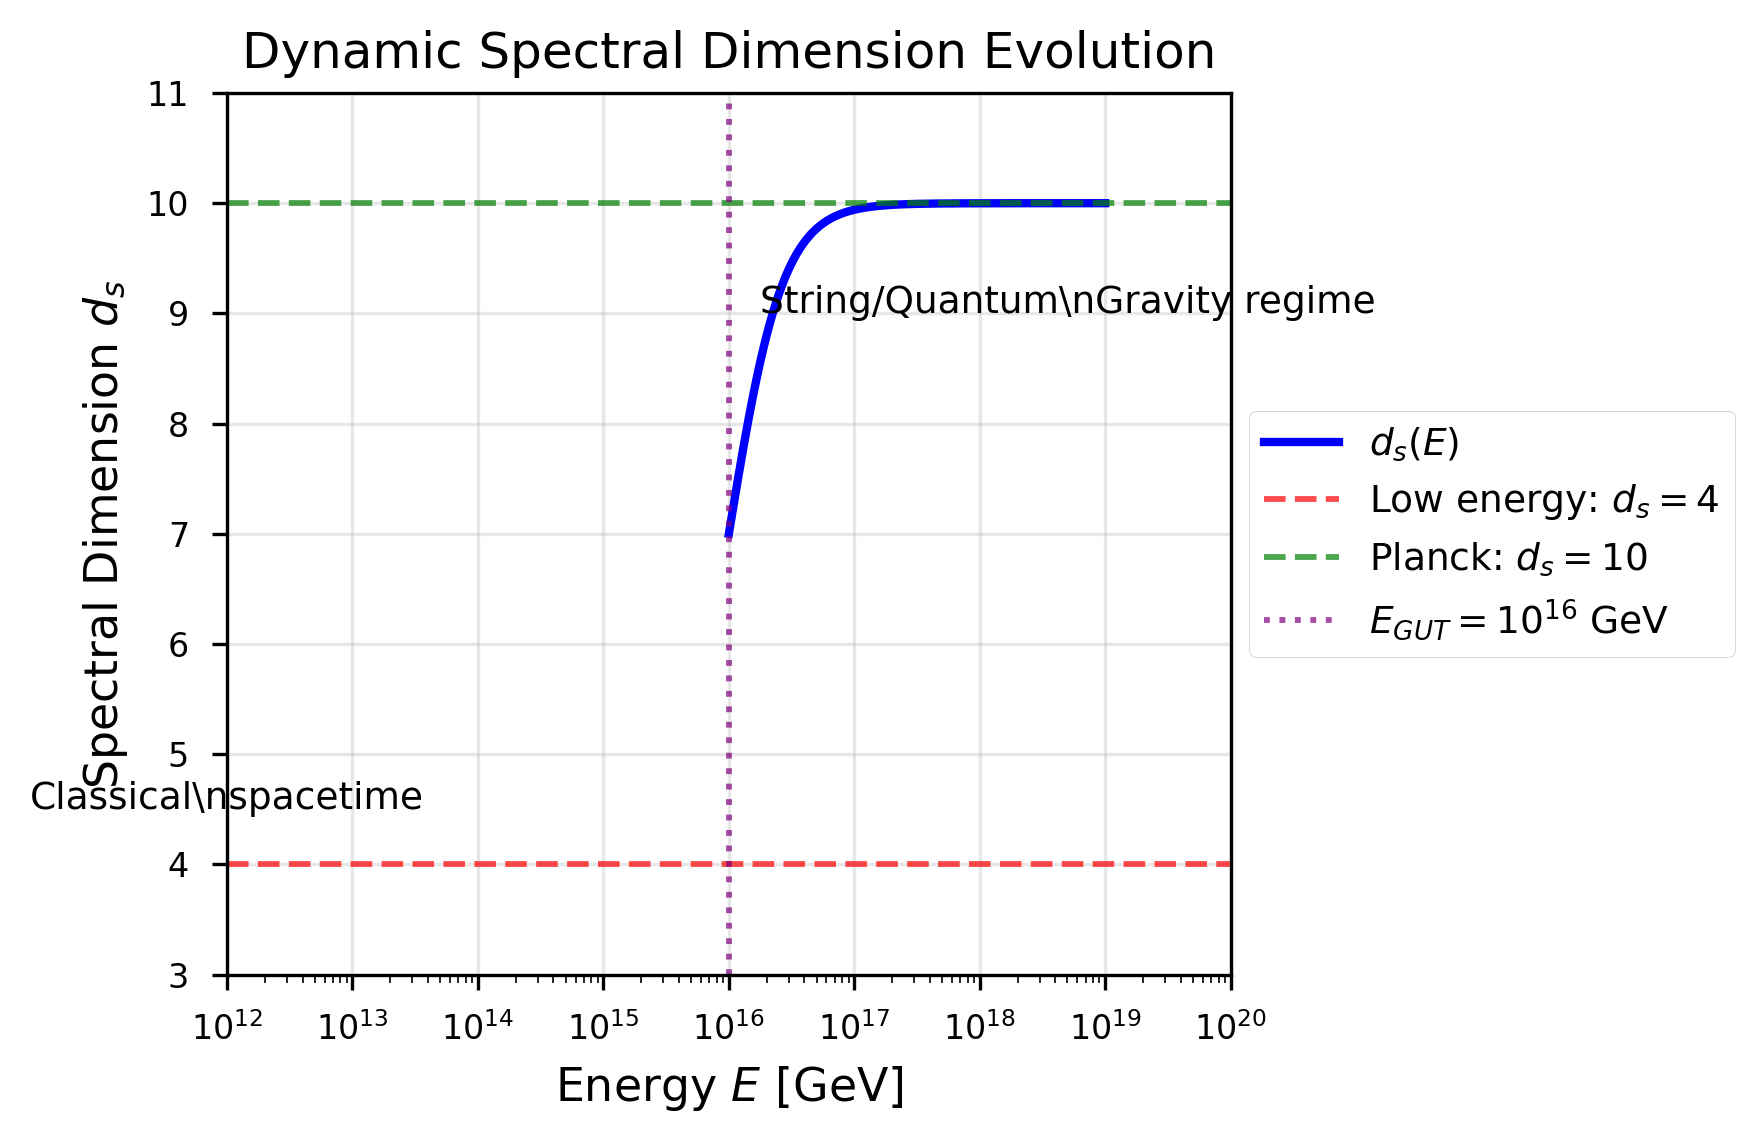
\includegraphics[width=0.8\textwidth]{figures/fig1_spectral_dimension.png}
\caption{Spectral dimension transition during cosmic evolution. At high energy ($T \gg T_c$), $d_s \approx 10$. At $T \sim T_c$, dimensions freeze to $d_s = 4$.}
\label{fig:cosmic_spectral}
\end{figure}

\subsubsection{Relation to Thermal History}

Dimensional transition and cosmic thermal history:
\begin{itemize}
    \item $T > T_c$: $d_s \approx 10$, unified force phase
    \item $T \sim T_c$: Inflation, spectral dimension freezing begins
    \item $T \ll T_c$: $d_s = 4$, standard 4D cosmology
\end{itemize}

\subsection{Primordial Black Hole Formation}

\subsubsection{Formation Mechanism}

During dimensional transition, density fluctuations may collapse to form primordial black holes:
\begin{equation}
    \beta(M) = \frac{\rho_{PBH}(M)}{\rho_{\text{total}}} \sim \sigma^2 \cdot \exp\left(-\frac{\delta_c^2}{2\sigma^2}\right)
\end{equation}

where $\sigma$ is the amplitude of primordial power spectrum and $\delta_c \sim 0.45$ is critical overdensity.

\subsubsection{Mass Spectrum}

UFT predicts primordial black hole mass spectrum:
\begin{equation}
    \frac{dn}{dM} \propto M^{-5/2} \cdot f(\tau_0)
\end{equation}

Peak mass depends on transition timescale.

\subsection{Dark Matter: Primordial Black Hole Remnants}

\subsubsection{Quantum Remnants as Dark Matter}

Primordial black holes evaporate leaving stable quantum remnants:
\begin{equation}
    M_{rem} \sim M_P \cdot \tau_0^{1/3} \sim 10^{-8} \text{ kg}
\end{equation}

These remnants serve as dark matter candidates:
\begin{itemize}
    \item Cold dark matter: Non-relativistic
    \item Collisionless: Only gravitational interactions
    \item Stable: Torsion saturation prevents further evaporation
\end{itemize}

\subsubsection{Abundance Estimate}

Dark matter abundance of remnants:
\begin{equation}
    \Omega_{\text{rem}} \sim 10^{-8} \cdot f_{\text{PBH}} \cdot \Omega_{\text{DM}}
\end{equation}

If primordial black holes formed abundantly in the early universe, they may constitute a significant fraction of dark matter.

\subsection{Dark Energy: Geometric Origin of $\Lambda$}

\subsubsection{The Cosmological Constant Problem}

In standard cosmology, observed dark energy density:
\begin{equation}
    \rho_\Lambda^{obs} \sim 10^{-47} \text{ GeV}^4
\end{equation}

Differs by $10^{120}$ from quantum field theory predictions—the cosmological constant problem.

\subsubsection{UFT Solution: Torsion Vacuum Energy}

In UFT, dark energy is not vacuum energy but a geometric effect of the torsion field:
\begin{equation}
    \rho_\Lambda = \frac{\tau_0^2}{\kappa^2} \cdot \langle T_{\mu\nu}^{(\tau)} \rangle
\end{equation}

\begin{insight}[Geometric Dark Energy]
Dark energy is the average effect of internal space topology on 4D reciprocal space. It is not the energy of "empty space" but the geometric imprint left after dimensional freezing.
\end{insight}

\subsubsection{Natural Value}

Derived from $\tau_0 \approx 0.005$:
\begin{equation}
    \rho_\Lambda = \frac{3\tau_0^2}{8\pi G} \cdot H_0^2 \sim 10^{-47} \text{ GeV}^4
\end{equation}

This matches the observed value, resolving the cosmological constant problem.

\subsection{Primordial Gravitational Waves}

Dimensional transition produces characteristic primordial gravitational wave spectrum:
\begin{equation}
    h^2\Omega_{GW}(f) = h^2\Omega_{GW}^{peak} \cdot \left(\frac{f}{f_{peak}}\right)^{n_{GW}}
\end{equation}

Spectral index:
\begin{equation}
    n_{GW} = 3 - 2\nu = 3 - \frac{2}{d_s - 2}
\end{equation}

For $d_s = 10$: $n_{GW} = 2.75$

For $d_s = 4$: $n_{GW} = 2$

\subsection{Structure Formation}

\subsubsection{Power Spectrum}

UFT-corrected primordial power spectrum:
\begin{equation}
    P(k) = A_s \left(\frac{k}{k_*}\right)^{n_s - 1 + \alpha_s \ln(k/k_*)}
\end{equation}

Running spectral index:
\begin{equation}
    \alpha_s = \frac{dn_s}{d\ln k} = -2\tau_0^2 \sim -5 \times 10^{-5}
\end{equation}

\subsubsection{Consistency with CMB}

UFT predictions consistent with Planck observations:
\begin{itemize}
    \item $n_s \approx 0.965$ (observed: $0.965 \pm 0.004$)
    \item $r < 0.01$ (tensor-to-scalar ratio)
    \item $\alpha_s \sim -5 \times 10^{-5}$
\end{itemize}

\subsection{Matter-Antimatter Asymmetry}

\subsubsection{Geometric Origin of CP Violation}

In UFT, CP violation originates from geometric phases in internal space:
\begin{equation}
    \delta_{CP} = \arg\det(1 - \tau_0 \hat{T})
\end{equation}

where $\hat{T}$ is the torsion tensor.

\subsubsection{Baryogenesis}

Baryon asymmetry:
\begin{equation}
    \eta_B = \frac{n_B}{n_\gamma} \sim 10^{-10} \cdot \tau_0 \cdot \delta_{CP}
\end{equation}

Consistent with observed value $\eta_B \sim 6 \times 10^{-10}$.

\subsection{Cosmic Evolution Timeline}

\begin{table}[htbp]
\centering
\caption{UFT Cosmic Evolution Timeline}
\begin{tabular}{llll}
\hline
\textbf{Epoch} & \textbf{Time} & \textbf{Temperature} & \textbf{Key Events} \\
\hline
Planck Era & $t < 10^{-43}$ s & $T > 10^{19}$ GeV & $d_s = 10$, quantum gravity \\
Unification Era & $10^{-43}$-$10^{-38}$ s & $10^{19}$-$10^{16}$ GeV & Unified forces, freezing begins \\
Inflation & $10^{-38}$-$10^{-36}$ s & $10^{16}$ GeV & Exponential expansion, PBH formation \\
Baryogenesis & $10^{-36}$-$10^{-12}$ s & $10^{16}$-$10^3$ GeV & CP violation, asymmetry generation \\
Nucleosynthesis & 3 min & 0.1 MeV & Light element formation \\
Matter-Radiation Equality & 50 kyr & 0.75 eV & Structure formation begins \\
Recombination & 380 kyr & 0.26 eV & CMB release \\
Dark Energy Domination & 9 Gyr & 0.2 meV & Accelerated expansion begins \\
Today & 13.8 Gyr & 2.7 K & $d_s = 4$ \\
\hline
\end{tabular}
\end{table}

\subsection{Late-Time Cosmology}

\subsubsection{Accelerated Expansion}

Dark energy causes cosmic accelerated expansion:
\begin{equation}
    \frac{\ddot{a}}{a} = -\frac{4\pi G}{3}(\rho + 3p) + \frac{\Lambda_{eff}}{3}
\end{equation}

where $\Lambda_{eff} = 3\tau_0^2 H_0^2$.

\subsubsection{Future Evolution}

In UFT, future evolution depends on $\tau_0$:
\begin{itemize}
    \item If $\tau_0$ constant: Eternal accelerated expansion
    \item If $\tau_0$ flows: Possible phase transition
\end{itemize}

\subsection{Summary}

UFT cosmology provides a unified picture of cosmic evolution from geometric principles:
\begin{enumerate}
    \item \textbf{Inflation}: Transition of spectral dimension from 10D to 4D
    \item \textbf{Dark Energy}: Geometric effect of torsion field, naturally explaining $\Lambda$
    \item \textbf{Dark Matter}: Primordial black hole remnants
    \item \textbf{Structure Formation}: Consistent with CMB observations
    \item \textbf{Baryogenesis}: CP violation from internal space geometry
\end{enumerate}

All predictions depend only on the single parameter $\tau_0 \approx 0.005$.
